\documentclass[xcolor=dvipsnames, USenglish]{beamer}  %notes=show to print them in the generated pdf
% Packages for a reasonable beamer session
\usepackage[T1]{fontenc}
%\usepackage[ansinew]{inputenc}
\usepackage[utf8]{inputenc}
\usepackage{textcomp}
\usepackage{lmodern}
\usepackage{csquotes}
\usepackage[english]{babel}
%\usepackage{babel}

\usepackage{graphicx}

\usepackage{amsmath}
\usepackage{amsfonts}
\usepackage{amssymb}
\usepackage{amsthm}
\usepackage{bm}

\usepackage{booktabs}
\usepackage{tabularx}

\usepackage{hyperref}

\usepackage{ellipsis}

% Additional packages
\usepackage{graphicx}
\usepackage{subfigure}
\usepackage{xcolor}
\usepackage{minted}

\usepackage[style=authoryear, backend=biber]{biblatex}
\setbeamertemplate{itemize/enumerate body begin}{\setlength{\leftmargini}{1.5em}}
\renewcommand*{\nameyeardelim}{\addcomma\addspace}
\addbibresource{\jobname.bib}
\renewcommand{\footnotesize}{\tiny}

\usepackage{tikz,pgf,calc}
%\usetikzlibrary{matrix, shapes, positioning, calc,
%  decorations.pathreplacing, shapes.geometric, arrows}
\usetikzlibrary{shapes.geometric, arrows, calc}
\tikzstyle{startstop} = [rectangle, rounded corners, minimum width=3cm, minimum height=1cm, text centered, text width=1.5cm, draw=black, fill=red!30]
\tikzstyle{io} = [trapezium, trapezium left angle=70, trapezium right angle=110, minimum width=3cm, minimum height=1cm, text centered, draw=black, fill=blue!30]
\tikzstyle{process} = [rectangle, minimum width=3cm, minimum height=1cm, text centered, draw=black, fill=orange!30]
\tikzstyle{decision} = [diamond, minimum width=3cm, minimum height=0.5cm, text centered, draw=black, fill=green!30]
\tikzstyle{arrow} = [thick,->,>=stealth]

%% References
\newlength\leftsidebar
\makeatletter
\setlength\leftsidebar{\beamer@leftsidebar}
\makeatother

\usepackage[absolute,overlay]{textpos}
\newenvironment{reference}[2]{%
  \begin{textblock*}{\textwidth}(\leftsidebar+#1,\paperheight-#2)
      \scriptsize\bgroup\color{red!50!black}}{\egroup\end{textblock*}}

% Path to graphics
\graphicspath{{../img/}}

% Sources
\usepackage{setspace}
\newcommand{\source}[1]{\begin{spacing}{0.5}{\fontsize{5}{6}\selectfont source: \itshape {#1}}\end{spacing}}
 % PACKAGES
% Collection of useful mathematical symbols and commands
% Calculus
\newcommand{\ud}{\mathrm{d}}
\newcommand{\pder}[2]{\frac{\partial{#1}}{\partial{#2}}}
\newcommand{\dpder}[2]{\frac{\partial^2{#1}}{\partial{#2^2}}}
\newcommand{\sderp}[3]{\frac{\partial^2{#1}}{\partial{#2}\partial{#3}}}
\newcommand{\tder}[2]{\frac{\ud{#1}}{\ud{#2}}}
\newcommand{\rot}[1]{\nabla \times {#1}}
\newcommand{\diver}[1]{\nabla \cdot {#1}}
\newcommand{\definter}[4]{\int_{#1}^{#2} {#3}\ud {#4}}
\newcommand{\inter}[2]{\int {#1}\ud {#2}}
\newcommand{\braket}[2]{\langle {#1} , {#2} \rangle}
% Misc
\newcommand{\eval}[1]{\Big |_{#1}}
\newcommand{\bset}[1]{\big\lbrace {#1} \big\rbrace}
\newcommand{\stimes}[2]{{#1}\!\times\!{#2}}
\newcommand{\trp}{\top}
\newcommand{\preup}[2]{{}^{#2}\!{#1}}

% Operators
\DeclareMathOperator*{\armin}{arg\,min}
\DeclareMathOperator*{\armax}{arg\,max}
\DeclareMathOperator*{\rank}{rank}
\DeclareMathOperator*{\cov}{cov}
\DeclareMathOperator*{\nullsp}{null}
% Logicals
\newcommand{\suchthat}{\big \backslash \;}
   % SYMBOLS

% ----------- Extra packages
\usepackage{../beamer_themes/beamerthemeEawag_blue} % Eawag style

% ----------- References used and shown
%\begin{filecontents}{\jobname.bib}

%\end{filecontents}


% ----------- Extra symbols
\newcommand{\ccov}[1]{{\color{red}k}\left(#1\right)}
\newcommand{\cmean}[1]{{\color{blue}m}\left(#1\right)}
\newcommand{\sm}{\scalebox{0.5}{-1}}

% ----------- New Environments
\newenvironment{Dview}{%
  \begin{exampleblock}{Data view}}{\end{exampleblock}}

%----------------
% title information
\title{Master Thesis}
\subtitle{Development of an Overland Flow Model Emulator}
\author[\texttt{sebastiano.rusca@eawag.ch}]{Sebastiano Rusca}
\institute[Eawag]{Eawag: Swiss Federal Institute of Aquatic Science
  and Technology}
\date[22.01.2018]{January 22, 2018}

% ====================================================================

\begin{document}

% ----------------
% Title frame
% load background for title
\setbeamertemplate{background}{
  
\includegraphics[width=\paperwidth,height=\paperheight]
  {../beamer_themes/background_title_blue.png}}
{ \setbeamertemplate{footline}{} % no footer on title
  \begin{frame}
    \titlepage
  \end{frame}
}
% load background for all other slides
\setbeamertemplate{background}{

\includegraphics[width=\paperwidth,height=\paperheight]
{../beamer_themes/background_slides_blue.png}}
%\setbeamertemplate{footline}[Sebastiano Rusca] % set footer
\addtocounter{framenumber}{-1}  % don't count title page

%%%%%%%%%%%%%%%%%%%%%%%%%%%%%%%%%%%%%%%%%%%%%%%
% WHAT IS EMULATION
\section{Introduction}

  \begin{frame}
    \frametitle{What is emulation?}
    \begin{itemize}
      \item \textbf{Emulator, aka surrogate model}: approximation model that mimic
      the behavior of a simulator model as closely as possible
      \begin{itemize}
        \item computationally cheaper to evaluate
        \item constructed with data driven, bottom-up approach
        \item internal states of the simulator model are lost
      \end{itemize}
    \end{itemize}

    \begin{figure}[b]
      \centering
        \subfigure[Simulator]{
          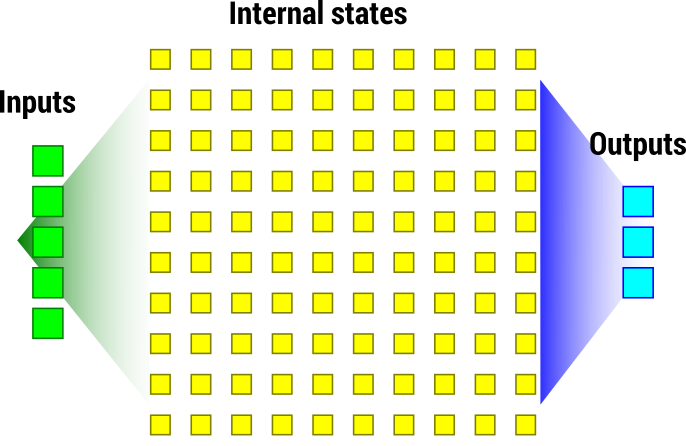
\includegraphics[width=0.4\textwidth]{img/simulator.png}
          }
        \subfigure[Emulator]{
           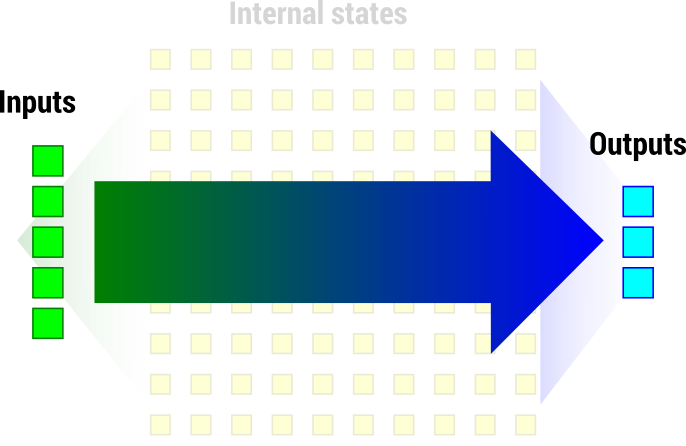
\includegraphics[width=0.4\textwidth]{img/emulator.png}
           }
    \end{figure}
    \source{"Model Order Reduction and Emulation." EmuMore's blog, January 20, 2018}
  \end{frame}

% As you can see from the title my master thesis deals with emulation.
% So first of all let's see what emulation is:
% Emulat

%%%%%%%%%%%%%%%%%%%%%%%%%%%%%%%%%%%%%%%%%%%%%%%%%%%%%%%%%%%%%%%%%%%%%%%%%%%%%%%%
% WHY OVERLAND FLOW

\section{Introduction}
  \begin{frame}
    \frametitle{Why overland flow?}
    \begin{itemize}
      \item very topical issue, also in Switzerland (e.g. Zofingen 2017)
      \item BAFU and cantons already dealing with the problem
      \item \textbf{simulators do a good job... but are still too slow}
    \end{itemize}
    
    \begin{figure}
      \centering
        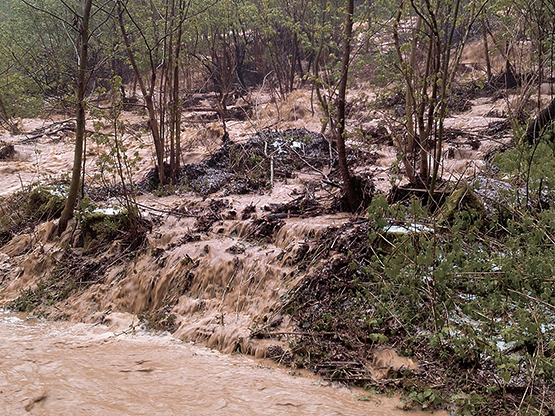
\includegraphics[width=0.25\textwidth]{img/overlandflow1.jpg}
        \quad
        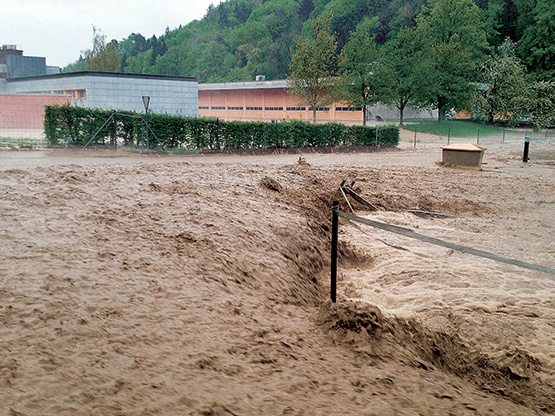
\includegraphics[width=0.25\textwidth]{img/overlandflow2.jpg}
        \\
        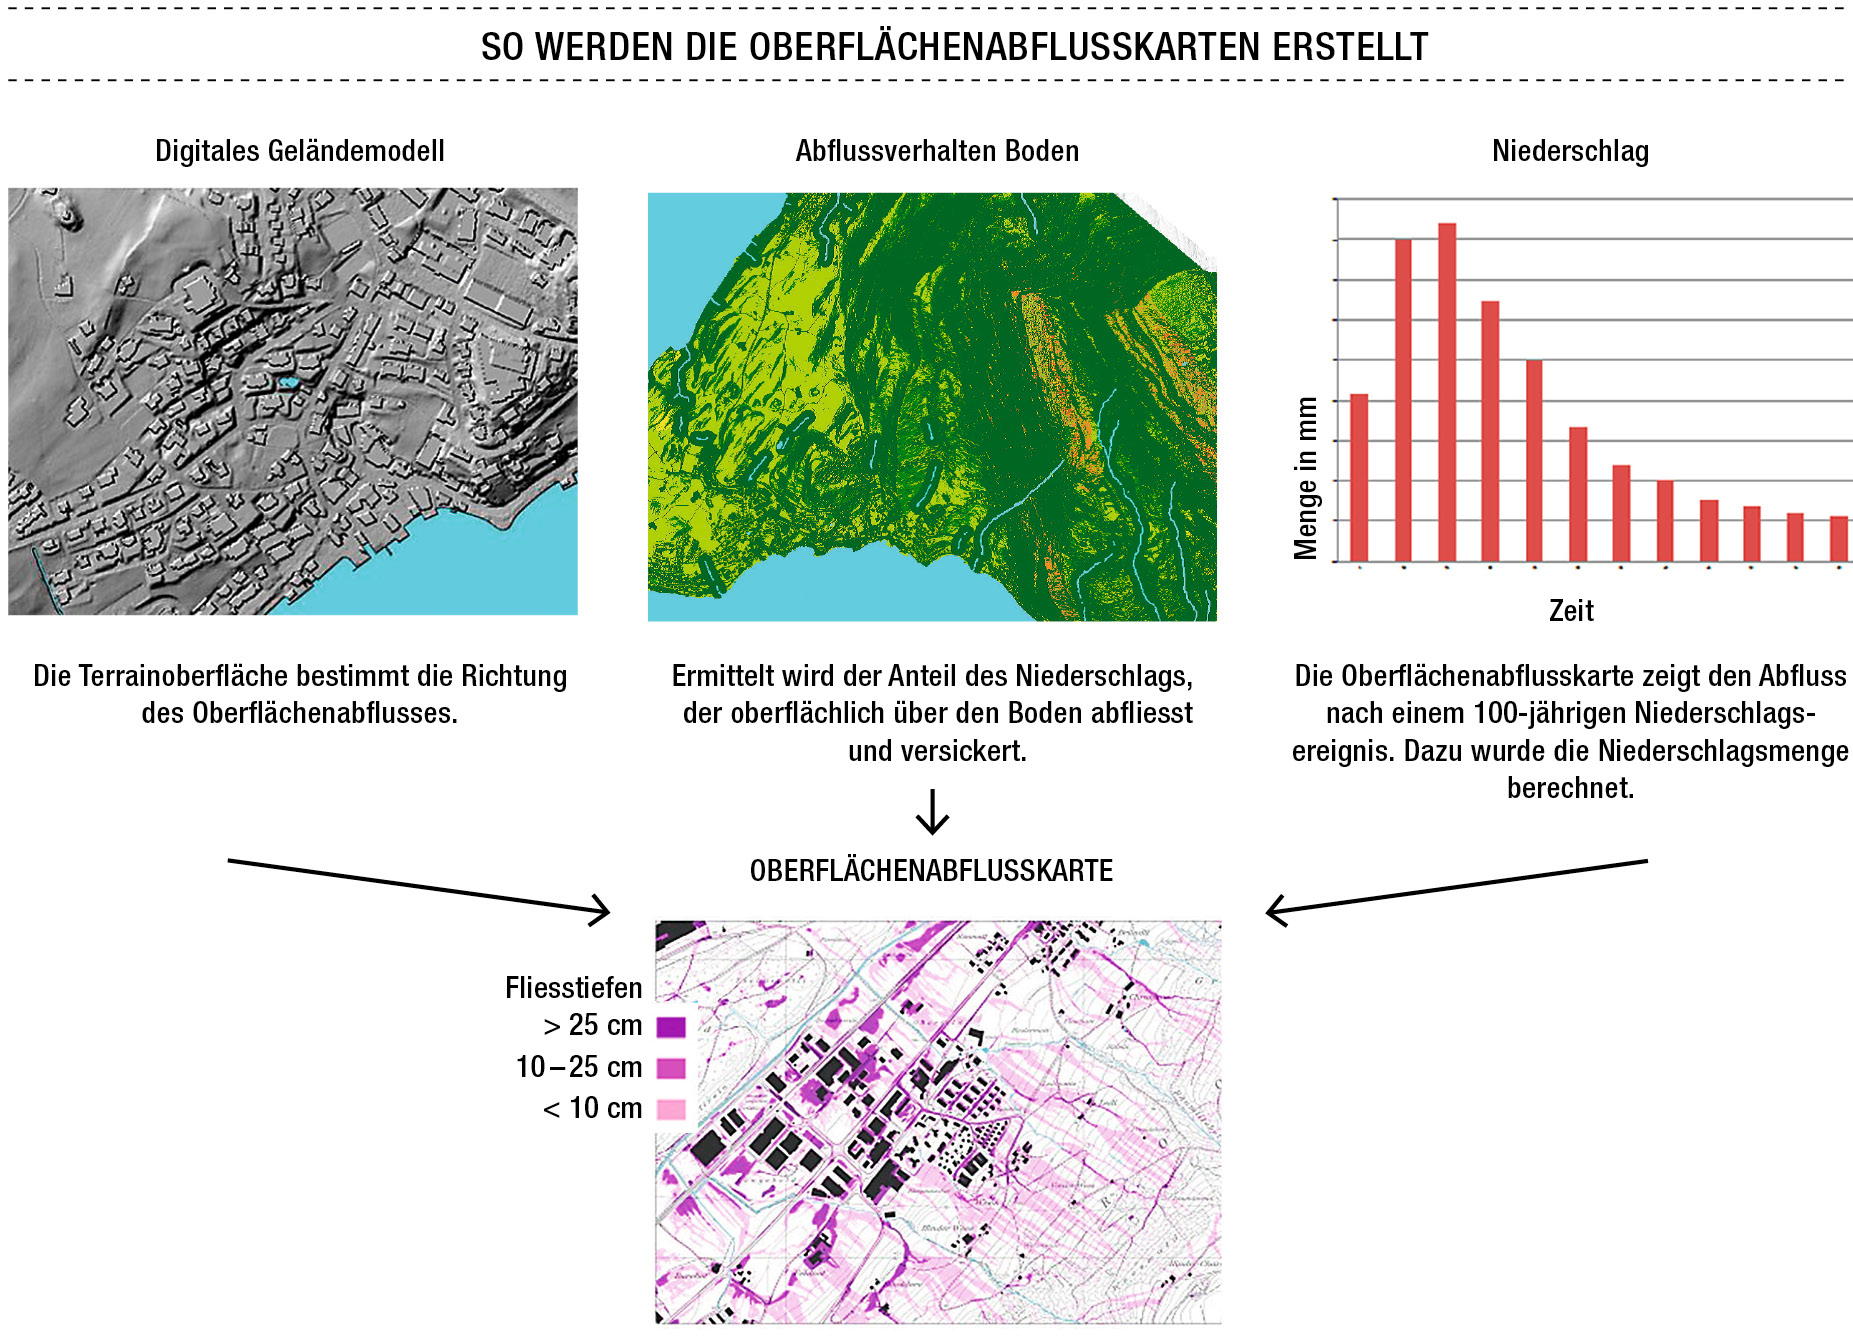
\includegraphics[width=0.25\textwidth]{img/overlandflow_map1.jpg}
        \quad
        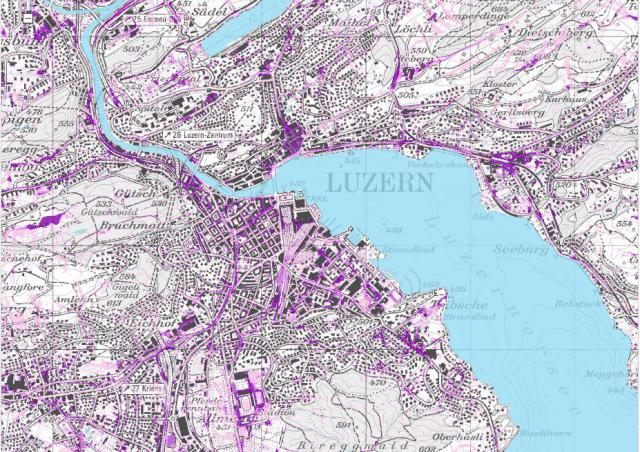
\includegraphics[width=0.25\textwidth]{img/overlandflow_map2.jpg}
    \end{figure}
    \source{Denzler, Lukas. "Quantensprung f\"ur die Pr\"avention von Wassersch\"aden." umwelt Magazine, 03/2017}
  \end{frame}

%%%%%%%%%%%%%%%%%%%%%%%%%%%%%%%%%%%%%%%%%%%%%%%%%%%%%%%%%%%%%%%%%%%%%%%%%%%%%%%%
% PROJECT CONCEPT: Idea and goals

\section{Project concept}
  \begin{frame}
    \frametitle{Project idea \& goals}
    \textbf{Idea: Emulate overland flow for a real Swiss case study}\\
    \begin{itemize}
      \item Obtain real topography and rain data (BAFU)
      \item Build specific emulators for the different study variables
      \item Assess their performance through comparison with historical datasets 
        (e.g. water depths, flow velocities, pictures)
    \end{itemize}
    \textbf{Goals}
    \begin{itemize}
      \item Design, dimension and optimize flooding mitigation structures making use of emulators
      \item Test effectiveness of emulator-based warning systems
      \item Assess suitability of locations for measurement sensors under various conditions
      \item Carry out water level uncertainty quantification
    \end{itemize}
  \end{frame}
  
%%%%%%%%%%%%%%%%%%%%%%%%%%%%%%%%%%%%%%%%%%%%%%%%%%%%%%%%%%%%%%%%%%%%%%%%%%%%%%%%
% FIRST EMULATOR: Problem definition

\section{1\textsuperscript{st} Emulator}
  \begin{frame}
  
    \frametitle{The weir equation: problem set-up}
    \begin{alertblock}{Weir equation}
      \setlength\abovedisplayskip{0pt}
      \begin{equation*}
        Q = \frac{2}{3}\: \textcolor{red}{\mu}\: B_w\: \sqrt{2g}\: h_{\"u}^{\textcolor{red}{a}}, \quad usu.\: \textcolor{red}{a = 3/2}
      \end{equation*}
    \end{alertblock}
    \begin{figure}[H]
      \centering
      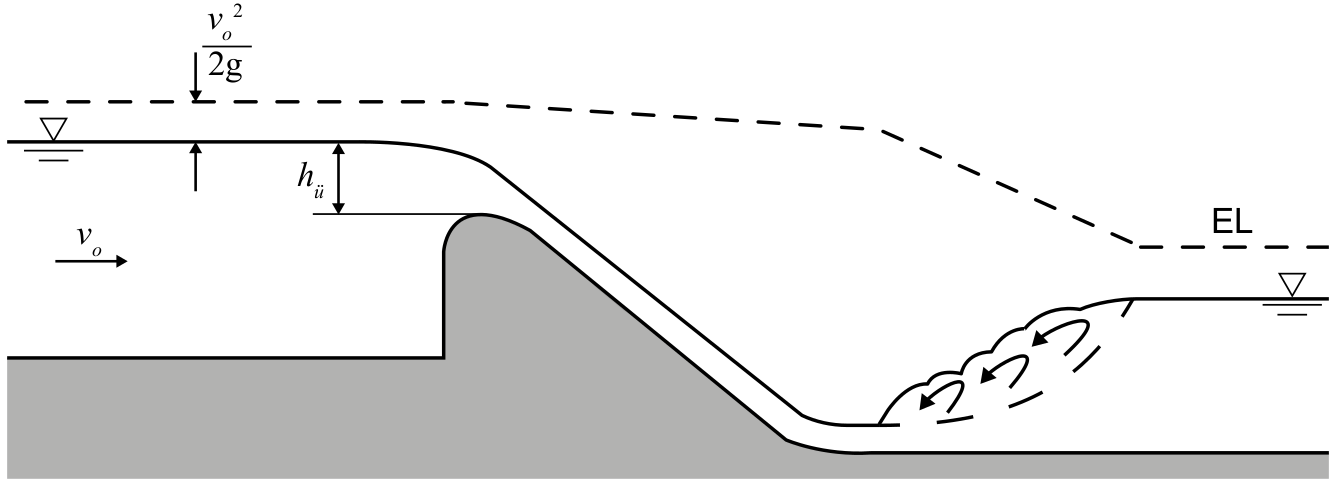
\includegraphics[width=0.7\textwidth]{img/weir_setup.png}
      \\
      $\boldsymbol{\mu:}$ \raisebox{-.2\height}{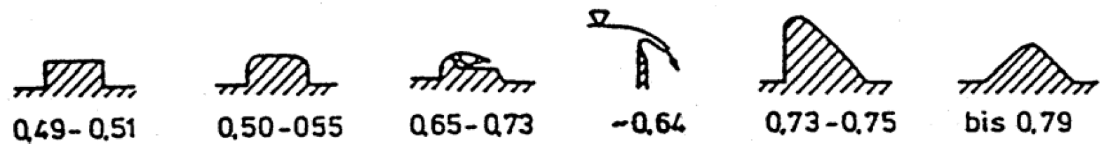
\includegraphics[width=0.6\textwidth]{img/weir_coefficients.png}}
    \end{figure}
    \source{Boes, Robert. "Wasserbau - Vorlesungsmanuskript." ETH Z\"urich - VAW, 2016.}

  \end{frame}
  

%%%%%%%%%%%%%%%%%%%%%%%%%%%%%%%%%%%%%%%%%%%%%%%%%%%%%%%%%%%%%%%%%%%%%%%%%%%%%%%%
% FIRST EMULATOR: The experiment

\section{1\textsuperscript{st} Emulator}
  \begin{frame}
  
    \frametitle{The weir equation: results}
    \begin{figure}[t]
      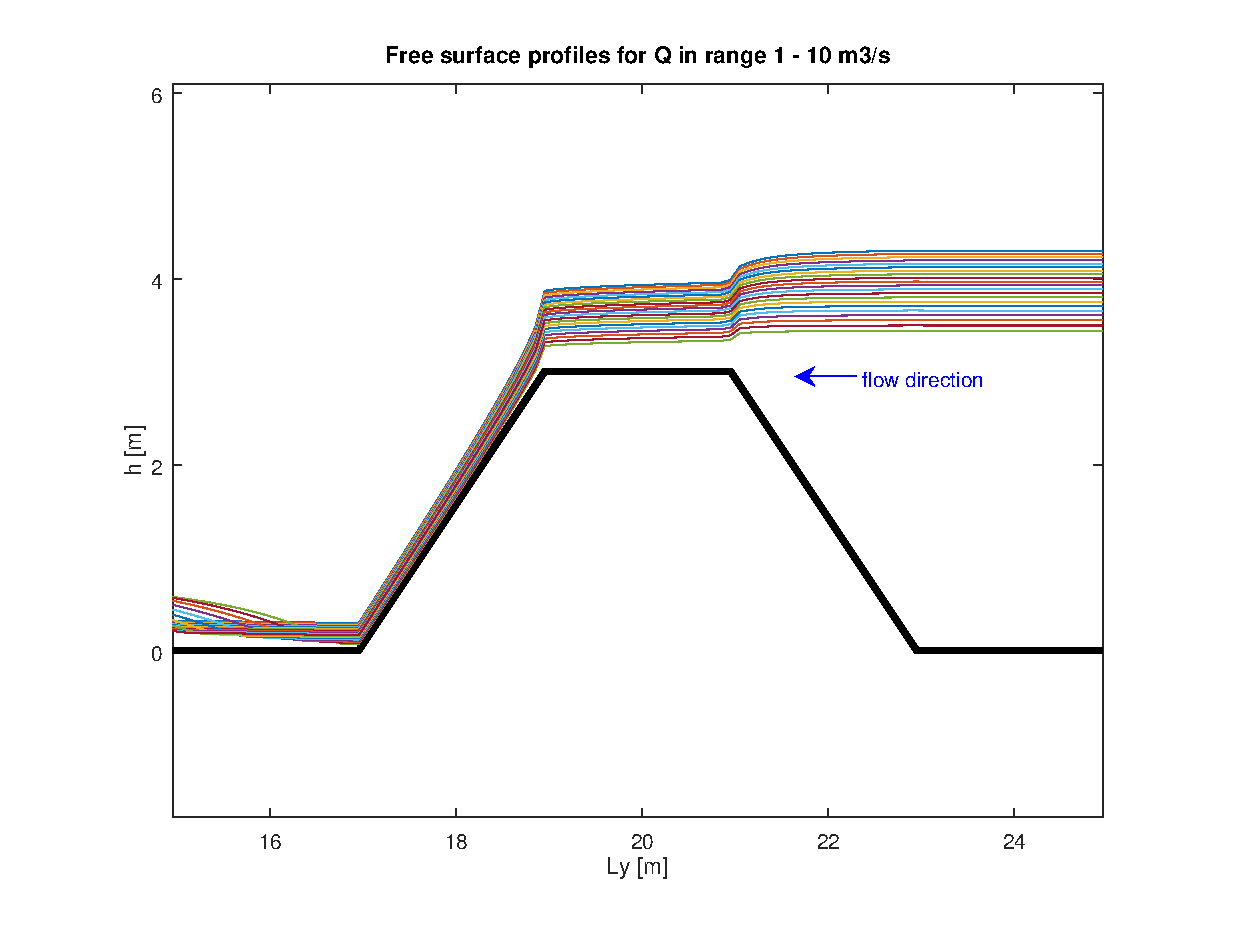
\includegraphics[width=0.5\textwidth]{img/free_surfaces.eps}
      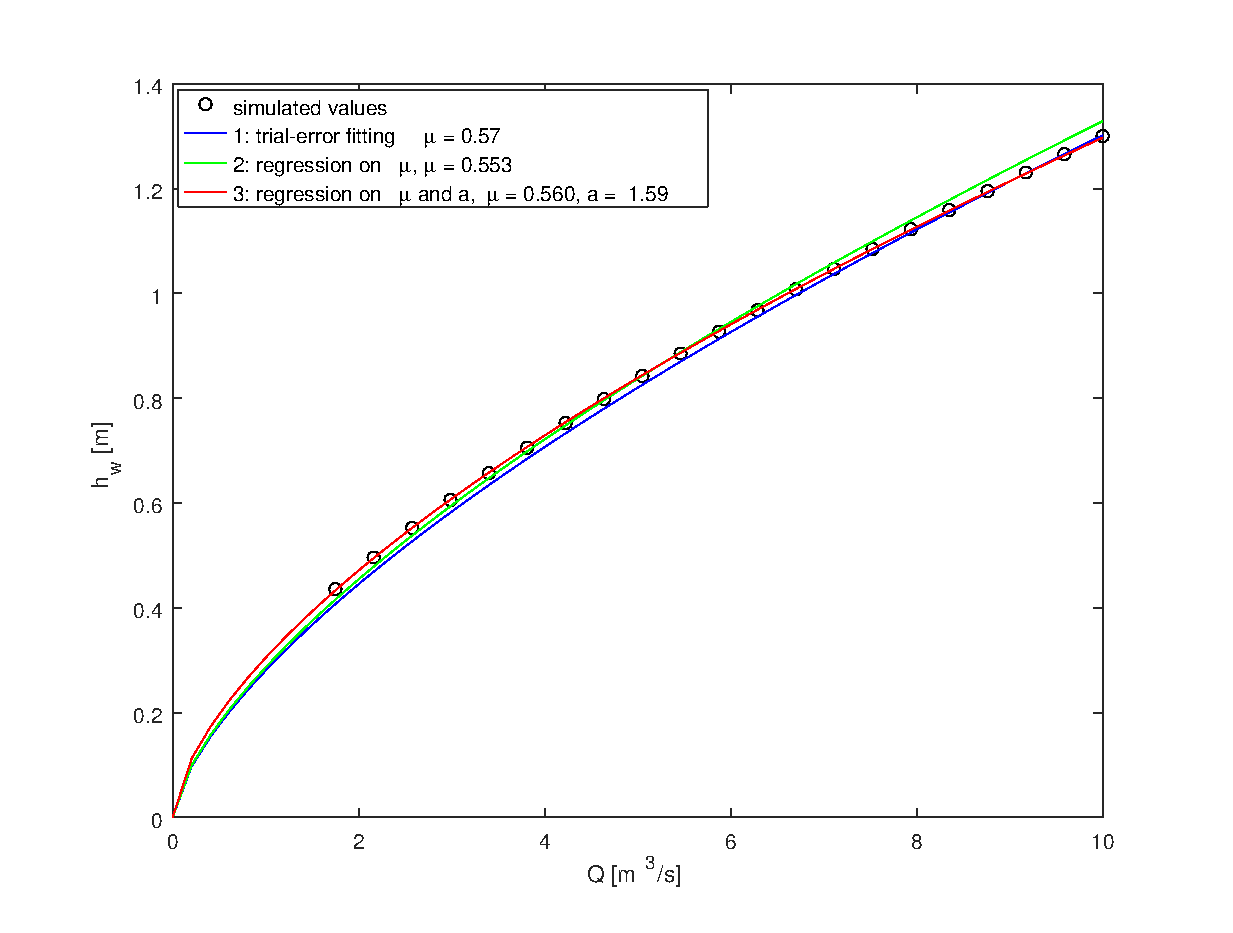
\includegraphics[width=0.5\textwidth]{img/points_interpolations.eps}
    \end{figure}

    \begin{table}
    \centering
       \begin{tabular}{lccc}
       \toprule
       \textbf{fitting method} & $\boldsymbol{\mu}$ &  \textbf{a} & \textbf{MSE}\\
       \midrule
       1: trial-error & 0.570 & 1.50 & 2.69E-04\\
       2: regression on $\mu$ & 0.553 & 1.50 & 2.36E-04\\
       3: regression on $\mu$ and a & 0.560 & 1.59 & 2.25E-06\\
       \bottomrule
       \end{tabular}
    \end{table}

  \end{frame}

%%%%%%%%%%%%%%%%%%%%%%%%%%%%%%%%%%%%%%%%%%%%%%%%%%%%%%%%%%%%%%%%%%%%%%%%%%%%%%%%
% NEXT STEPS

\section{Outlook}
  \begin{frame}
    \frametitle{Next steps}
    \begin{figure}
      \centering
      \subfigure[floodX case study]{
        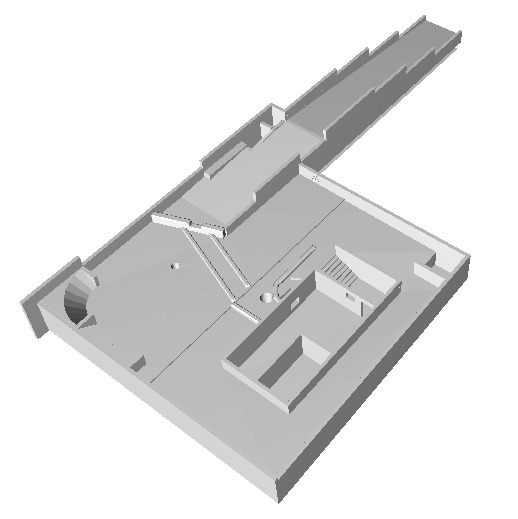
\includegraphics[width=0.3\textwidth]{img/floodx.png}
      }
      \subfigure[Coimbra case study]{
        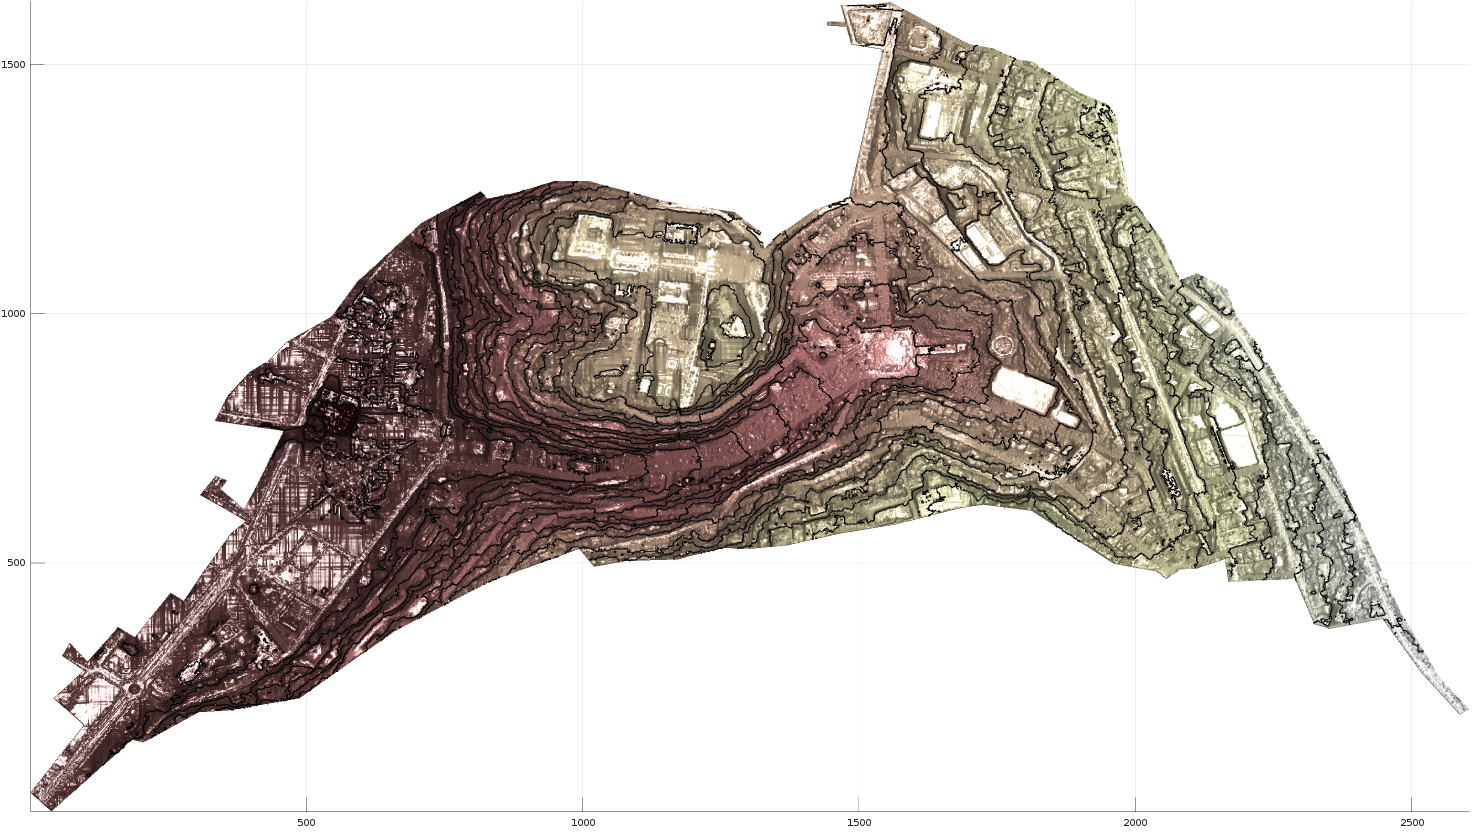
\includegraphics[width=0.5\textwidth]{img/coimbra.png}
      }
      \subfigure[Swiss case study]{
        
\includegraphics[width=0.3\textwidth]{img/question.png}
      }
    \end{figure}
  
  \end{frame}
\end{document}

